\chapter{Simulation model}\label{ch:model}

From the specifications described in \chref{ch:specs} we have defined the
following modules that compound the model:
\begin{description}
	\item[Floorplan] The \emph{network} representing the 2D floorplan and
		containing the users.
	\item[User] A \emph{submodule} representing a user in the system.
\end{description}

Additionally, to end the simulation when all reachable users have been infected
and to collect some statistics about the entire floorplan, we have added an
\standout{Oracle} module.

\section{Parameters}\label{sec:parameters}

\begin{itemize}
	\item \standout{Floorplan}:
		\begin{description}
			\item[userCount] \textit{(int)} The number \(N\) of
				users inside the network (default: \code{100}).
			\item[sizeX] \textit{(meters)} The horizontal size of
				the floorplan (default: \code{150m}).
			\item[sizeY] \textit{(meters)} The vertical size of the
				floorplan (default: \code{150m}).
			\item[indexStartingNode] \textit{(int distribution)} A
				random number generated from a distribution to
				select a random user to broadcast the message at
				the start of the simulation (default:
				\code{intuniform(0, userCount-1)}).
		\end{description}
	\item \standout{User}:
		\begin{description}
			\item[posX] \textit{(meters)} The X-axis position of the
				user in the floorplan (default: set by Floorplan
				as \code{uniform(0m, sizeX)}).
			\item[posY] \textit{(meters)} The Y-axis position of the
				user in the floorplan (default: set by Floorplan
				as \code{uniform(0m, sizeY)}).
			\item[sendOnStart] \textit{(bool)} Specifies if the user
				should send out the message at the start of
				simulation (default: \code{false}).
			\item[slotDuration] \textit{(seconds)} The duration of a
				time slot (default: \code{1s}).
			\item[broadcastRadius] \textit{(meters)} The broadcast
				radius \(R\) (default: \code{20m}).
			\item[hearWindow] \textit{(int)} The time window of
				\(T\) slots that the user should wait before
				relaying the message (default: \code{5}).
			\item[maxCopies] \textit{(int)} The maximum number of
				copies \(m\) that the user can receive to
				decide to relay the message (default: \code{3}).
				Note that our model counts also the first
				message as a ``copy'', but this is not an issue
				since the problem defined in \chref{ch:specs}
				says ``less than \(m\) copies'' (\emph{strict}
				constraint) while here we talk about the
				``maximum number of copies (including first
				message)'' (\emph{loose} constraint).
			\item[relayDelay] \textit{(int distribution)} The number
				of time slots \(\delta\) to add to the time
				window \(T\) before relaying the message
				(default: \code{intuniform(0, 3)}).
		\end{description}
	\item \standout{Oracle}:
		\begin{description}
			\item[slotDuration] \textit{(seconds)} The duration of a
				time slot. It should be equal to
				\code{User.slotDuration}.
			\item[timeout] \textit{(int)} The number of time slots
				with no network activity the oracle must wait
				before stopping the simulation. It should be
				\(\geq T+\max(\delta)\).
		\end{description}
\end{itemize}

\begin{tcolorbox}[title=Note]
	Since users only operates at time slot intervals, the parameter
	\code{slotDuration} does not affect the behavior and the performance of
	the network in any way. The only effect is that times \exgratia{total
	broadcast time} are scaled, so we will fix this parameter to \(1s\). In
	this way, each second of simulation time represents a time slot and the
	analysis become easier since, by default, \omnetpp{} records emitted
	signals with the timestamp at with emission occur.

	Of course this is not the case in a real system (probably each slot is
	much more shorter than 1 second) but this decision will not break any
	consideration made by our analysis, except for the time scaling effect.

	In the following we may use the terms ``1 slot'' and ``1 second''
	interchangeably.
\end{tcolorbox}

\section{Collected statistics}\label{sec:statistics}

All \code{@statistic} are defined in the \code{Floorplan} network's NED file and
they are collected using the \omnetpp{} signaling system by the \code{Oracle}
and the \code{User} modules.

The following statistics are collected by the \code{Oracle} module and are
related to the entire \code{Floorplan} network:
\begin{description}
	\item[activityTime] When a user perform some ``activity'' \idest{receive
		or send a message, excluding self messages} the Oracle signals
		the simulation time of the event. The last value signaled is
		recorded and represents the total broadcast time (regardless of
		whether all users have been reached or not).
	\item[coveredUsers] The number of users infected \idest{those who
		successfully heard the message}. A value with timestamp is
		recorded in each slot along with the sum of all values (the
		total number of infected users at the end of the simulation).
	\item[rcvMsgsPerSlot] For each slot, the number of messages that have
		been successfully heard by users. Also general statistics
		\idest{mean, stddev, min, max, \etc} are recorded.
	\item[sntMsgsPerSlot] For each slot, the number of users who sent out
		the message. General statistics are also recorded.
\end{description}

The following statistics are collecte by the \code{User} module and are mainly
related to the single user in the simulation:
\begin{description}
	\item[collisions] The number of collision registered by the user.
		General statistics are collected along with the sum of all
		collisions in the entire network.
	\item[copies] The number of copies of the message successfully heard by
		the user during the time window between the reception of the
		message and the time at which the user relays it. General
		statistics are collected.
	\item[reachedUsers] When a user relays the message, it signals the
		number of users reached (regardless of whether they correctly
		hear the message or not). General statistics are collected.
\end{description}

\section{Model implementation}\label{sec:implementation}

Implementation of the \code{User} and \code{Oracle} modules are available in the
\code{src/} folder. The definition of the \code{Floorplan} network is available
in the \code{simulations/} folder, along with configuration files for tests
(\code{tests.ini}) and simulations used for the analysis
(\code{simulations.ini}).

The main module of our implementation is the \code{User} module, so we will
start discussing it first.

\figref{fig:userfsm} shows the finite-state machine (FSM) diagram of the
\code{User} module. Exchanged messages are represented in upper case. Additional
conditions to move from one state to another are shown inside square brackets.
Operations on counter variables (\code{counter} and \code{slotcount}) are shown
in \textit{italic}. Symbols \(m\), \(T\) and \(\delta\) represents,
respectively, the parameters \code{maxCopies}, \code{hearWindow} and
\code{relayDelay}.

\begin{figure}[htb]
	\centering
	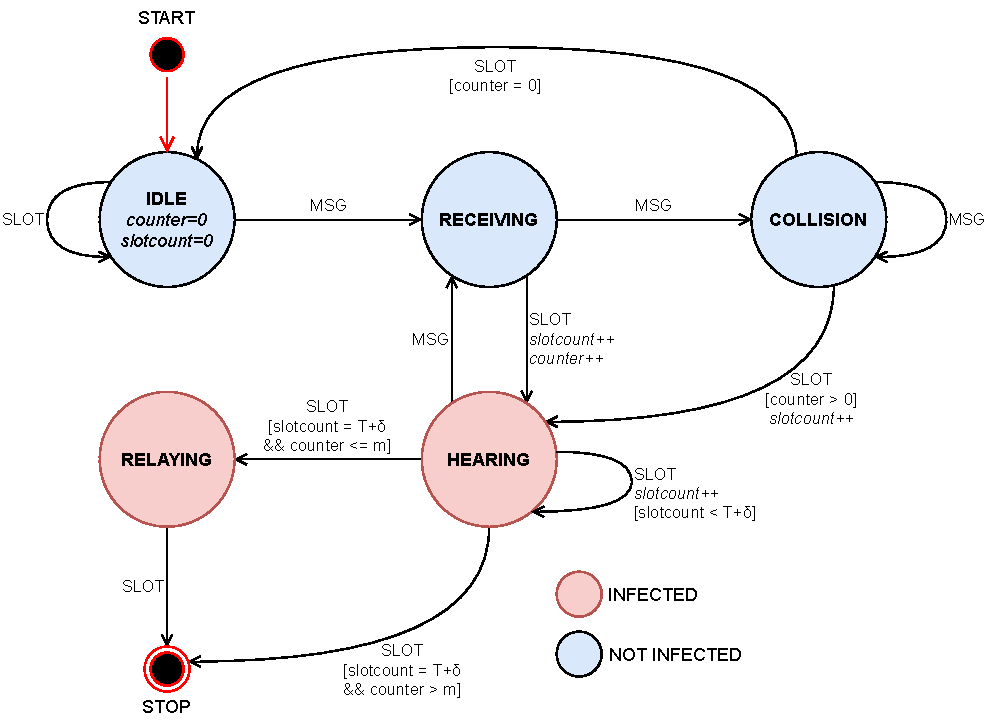
\includegraphics[width=\textwidth]{img/userfsm}
	\caption{FSM diagram of the \code{User} module}\label{fig:userfsm}
\end{figure}

We note that in our implementation of the \code{User} module, the transmission
of the message exchanged between users (\code{MSG}) does not really occupies an
entire slot (we have set its propagation delay equal to
\(\textrm{slotDuration}/2\)) in order to guarantee the order of events:
exchanged messages between users always come before self-messages used for
slotting, thus ensuring that the message is received in the current slot. In any
case, actual actions that the user should perform after a message is received
always take place in the next time slot.

The \code{Oracle} module is just a simple module that collects some ``global''
statistics and stops the simulation when no more activity is present in the
network \idest{no user is going to relay the message}. Users informs the oracle
of their actions via direct cross-module calls.

Note that also the oracle performs slotting in order to properly be synchronized
with all other nodes when emitting statistic signals and to decrease the
\code{timeout} variable if no activity has been seen in the network during the
last slot. In order to ensure that the oracle always runs after all other nodes,
its self-messages used for slotting have been set to a lower scheduling
priority.

\figref{fig:snapshot} shows a snapshot of our model running in the \omnetpp{} QT
environment at \(t = 16s\) (event \#896) with the configuration ``DocExample''
(\code{tests.ini}). \code{IDLE} and \code{RECEIVING} states are represented by
the \textcolor{idle}{\textbf{gray}} color; \code{HEARING} state is represented
by the \textcolor{hearing}{\textbf{blue}} color; \code{COLLISION} state is
represented by the \textcolor{collision}{\textbf{red}} color; \code{RELAYING}
state is represented by a circle surrounding the user that shows the broadcast
radius (only users inside this circle will be reached); Stopped users are
represented by the \textcolor{relayed}{\textbf{green}} color.

\begin{figure}[htb]
	\centering
	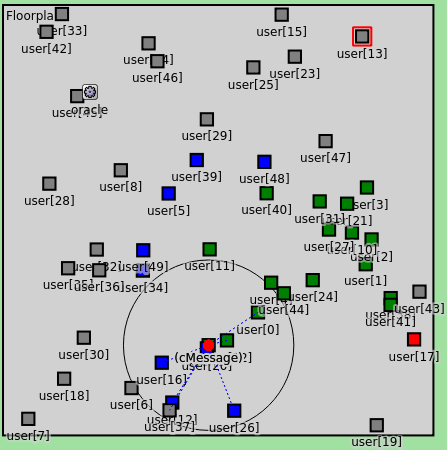
\includegraphics[width=\textwidth]{img/snapshot}
	\caption{Snapshot of our model running with the configuration
	``DocExample'' in the \omnetpp{} QT environment}\label{fig:snapshot}
\end{figure}

\section{Model verification}\label{sec:verification}

To ensure that our implementation does not contains bug and correctly implements
the model we have performed various tests:
\begin{description}
	\item[Memory Check] We have used Valgrind on all tests defined in
		\code{tests.ini} to verify that there were no bad memory
		accesses and memory leaks.
	\item[Graphical Test] We have run the ``Simple'' configuration in the
		\omnetpp{} QT environment to check visually that the network
		works as expected. We have also collected statistics for these
		runs and checked that they are consistent with what we have seen
		in the graphical environment. This test has been also performed
		for the ``DocExample'' configuration, as shown in
		\figref{fig:snapshot}.
	\item[Step-by-Step Debug] We have also debugged the ``Simple''
		configuration step-by-step to check that our code takes the
		expected code path.
	\item[Event Trace Check] For the ``Simple'' configuration we have also
		logged and verified the event trace in order to ensure that
		events are scheduled in the correct order.
	\item[Deterministic Test] We have run the ``Deterministic''
		configuration in multiple repetitions and verified that the
		results were the same for all runs.
	\item[Degeneracy Test] We have run the ``UserDegeneracy'' configuration
		and tested that the network simply does nothing and all recorded
		statistics are equal to zero with zero users, while only a
		message is sent (not heard by anyone) with one user. We have run
		the ``NoRadius'' configuration and checked that the first user
		sending the message is not able to reach anyone. We have run the
		``Unreachable'' configuration (two users at long distance) and
		verified that the user sending out the message is not able to
		reach the other.
	\item[Continuity Test] We have run the ``Continuity'' configuration and
		verified that all the measured quantities increase as the number
		of users increases. As an example, in \figref{fig:continuity}
		we can see that the total broadcast time and the number of
		collisions increase with the number of users in the network. We
		note that the test has been performed by varying the total
		number of user but keeping the user density fixed \idest{by
		keeping the \(\frac{N}{A}\) ration fixed}.
\end{description}

\begin{figure}[htb]
	\centering
	\verb|\includegraphics[width=\textwidth]{img/continuity}|
	\caption{Continuity test for the total broadcast time and the total
	number of collisions when the number of users in the network
	increases}\label{fig:continuity}
\end{figure}

